%*******************************************************************************
%****************************** Third Chapter *********************************
%*******************************************************************************

\chapter{Background}

\ifpdf
    \graphicspath{{Chapter3/Figs/Raster/}{Chapter3/Figs/PDF/}{Chapter3/Figs/}}
\else
    \graphicspath{{Chapter3/Figs/Vector/}{Chapter3/Figs/}}
\fi

%********************************** %First Section  **************************************
\section{Introduction}

A comprehensive background on the key concepts that the method presented in this thesis is based on is essential for understanding its context and significance. Any physical or mathematical principles that might affect the performance of the method should also be understood. The previous chapter outlined some of the problems faced when attempting to segment cancer cells given a 3D live cell environment. These included autofocus fluctuations of the microscope and limits on light absorption by cells. This chapter gives some detail on topics including the GFP distribution within the cells, which plays a key role in the pre-processing method, basic image processing and segmentation and how these techniques are used in CellProfiler and other segmentation software packages, and finally an introduction to the brightfield method on which the current method is based.

\section{Cell microscopy, optical structure, and GFP distributions}

Under a microscope, the visible parts of a cell, the optical properties of edges, and colours observed depend on the materials that it contains. A typical human cell is colourless and transparent [ref], but when light passes tangentially through the cell wall, it can be blocked and give the appearance of a dark edge. This leads to a projected (2D) shape under the microscope. This shape is a closed curve and thus has an interior (the material within the cell) and an exterior (the background). This is an assumption made throughout the segmentation process, since it is not possible for the cell to be an open shape. This is useful for segmentation, because there is a natural boundary that allows the recognition to be restricted to closed curves made up of dark edges.

Cells can move in response to chemical stimuli [ref]. In order to move in their environment, a cell can change tension in its outer wall and form protrusions that stretch in the direction of a stimulus [ref]. This can allow the cell to propel itself and follow chemical gradients. These protrusions, if they can be measured, provide useful information about the behaviour of the cell in response to any agents that have been added to the system as part of the experiment. The microfluidics environment was designed with the addition of chemical agents in mind. Even without added stimuli, the purpose of the experiment is to be able to observe the cells moving and allow for their shapes to be measured. Accurate recognition of cell protrusions is a key aim of this study. Without it, cell behaviour cannot be judged in changing conditions.

Cells can be marked by injecting a variety of fluorescent proteins into different parts of their internal structure such as the internal cytosol, the cell membrane, and the nucleus. A common protein used is known as GFP, or Green Fluorescent Protein. It is usually expressed in the cytosol, a clear fluid surrounding the nucleus, occupying the bulk of the cell, but not the membrane or the nucleus [ref]. When a 3D reconstruction is created using a confocal microscope, this distribution of GFP will appear as a single bulk shape with a gap at the location of the nucleus. It notably does not contain information about the extremities of the cell such as protrusions. It can also be expressed in the cell membrane, leading to a hollow 3D shape that shows clearly the extremities of the cell.

\begin{figure}[h!]
 \centering
 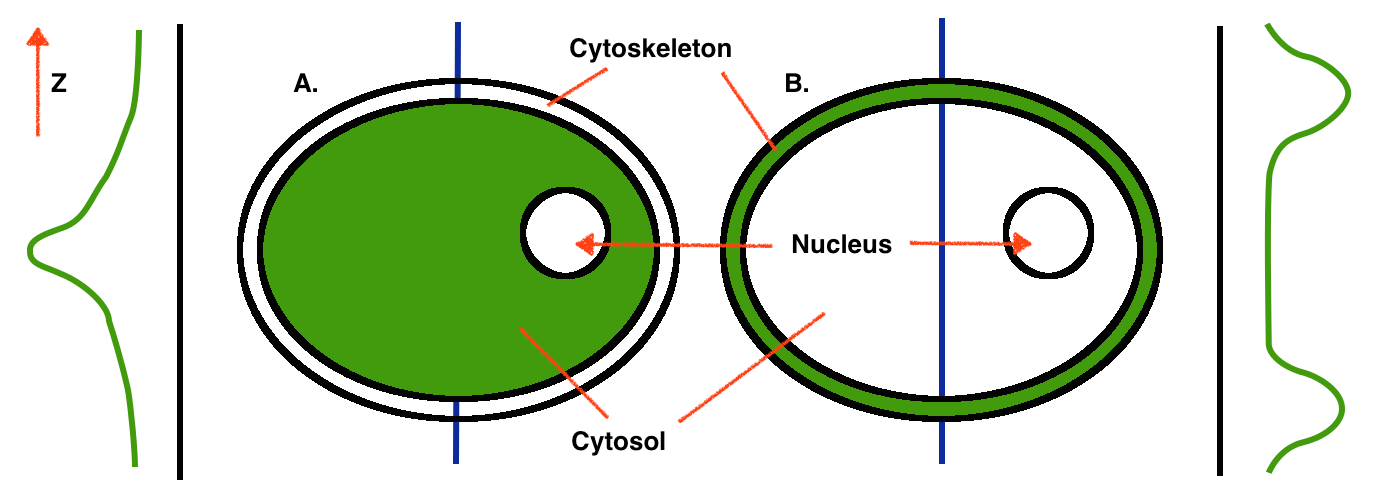
\includegraphics[width=0.9\textwidth]{301_gfp_distributions}
 \caption[Possible GFP distributions]{
	Different parts of a cell are composed of different materials that can be made to bind with fluorescent proteins such as GFP to highlight the cell structure in a microscope image. For example the rigid skeleton of the cell and the outer wall are composed primarily of actin filaments. The wall is marked as the cytoskeleton, but in reality it extends throughout the cell in filaments. This method relies on a consistent formation of the GFP inside a cell. It could be made to bind with the cytoskeleton, such as in B. This would produce a vertical intensity profile along the blue line similar to the plot on the right with two peaks. This method expects a single peaks for the centre of the cell, such as in A, since this type of staining is used in the experiemnts. The method would have to be modified to account for these types of changes. Note the lack of GFP expressed in the nucleus.
 }
 \label{fig:gfpdistributions}
\end{figure}

\section{Image processing and segmentation}

One of the most important features that can be extracted from an image is the location of edges. They delimit objects and provide evidence of texture within an object. An edge is defined as an intensity discontinuity in one dimension. Crossing the edge, the intensity can be plotted and represented as a mathematical relationship between the intensity and the path taken. Movement across a thin dark edge will show a decrease in intensity followed by a subsequent increase once the edge is passed. This is dependent on the image, but a robust mathematical model allows edges in a set of images to found quickly and reliably if it is general enough. The ability to rapidly find edges in an image is a key tool in a segmentation program, since this is the most certain way of locating objects. An example of a widely used edge detection method is called the Canny filter. Proposed by John Canny in his 1986 paper, A Computational Approach To Edge Detection [italic]. It works by first smoothing the image to reduce noise, finding the intensity gradients of the image (edges will show a high intensity gradient), suppressing points with less than the maximum gradient, along with applying an absolute intensity threshold, and finally joining potential edge segments by removing those not connected to strong edge segments. Other features such as corners can be modelled as superpositions of the simple edges in different orientations.

\begin{figure}[h!]
 \centering
 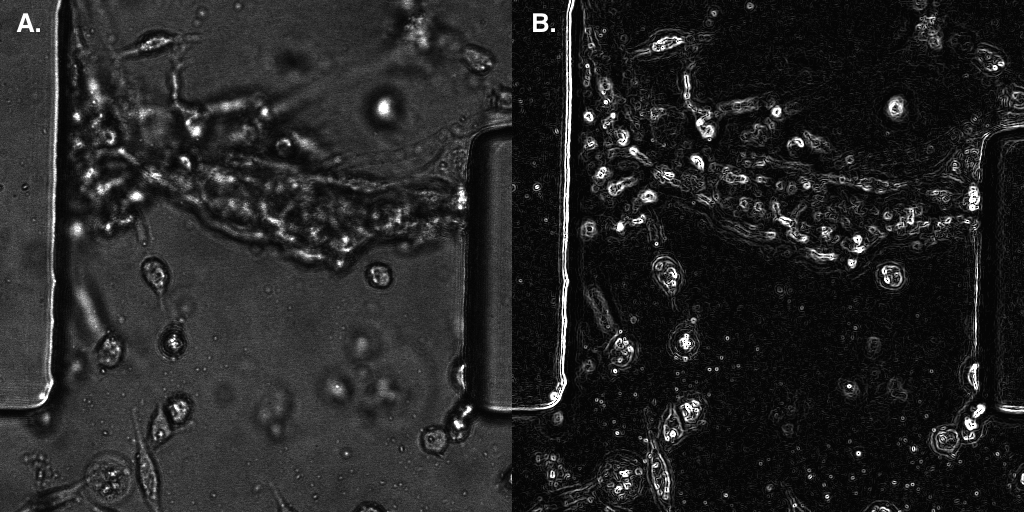
\includegraphics[width=0.9\textwidth]{302_sample_canny}
 \caption[Example of the Canny edge filter]{
 	By analysing the intensity gradients in an image, the Canny edge filter highlights the points with the highest intensity discontinuities. These appear as the edges of the image in the above example.
 }
 \label{fig:canny}
\end{figure}

Here is a list of steps to complete the Canny algorithm:
\begin{enumerate}
	\item The image to be processed in smoothed using a Gaussian kernel of the form, with size $2k + 1$:
	$$ H_{ij} = \frac{1}{2 \pi \sigma^2} exp \left( -\frac{(i - k - 1)^2 + (j - k - 1)^2}{2 \sigma^2} \right) $$
	\item Find the intensity gradient of the image in 2D (both magnitude and direction).
	$$ G = \sqrt{G^2_x + G^2_y} $$
	$$ \Theta = atan2(G_y, G_x) $$
	\item Perform non-maximal suppression on the resulting gradient image. This is done in two stages:
	\begin{enumerate}
		\item Compare the edge response of each pixel to the its nearest neighbours in each gradient direction.
		\item If the value of the pixel is greater than its neighbours, preserve it, else suppress it.
	\end{enumerate}
	\item To suppress any pixels left over after non-maximal suppression due to noise or other random colour variations, apply a double threshold to the resulting image. This is normally done using the Otsu method [ref], which minimises the variance between two classes of pixels, a Foreground, or cell objects, and the Background.
	\item Lastly, complete any broken edges using Hysteresis. This processing searches for objects in the image and attempts to incorporate weak edge pixels into the final edge image. This is done by looking at all 8 neighbour pixels for a weak edge. If at least one strong edge pixel is found, the weak edge pixel will be preserved.
\end{enumerate}

Another tool for recognition is the blob detector. A ``blob" is a technical term meaning an contiguous (interconnected) region of uniform (similar) colour. This could indicate a solid object or a region of background. Depending on the type of imaging, blobs that represent objects can either be light or dark, but both can be found by modelling the region as a 2D intensity discontinuity. This can be represented mathematically as a 2D Gaussian of arbitrary, but fixed, radius. Such a modelling function can then be convolved with the image in a similar manner to simple edges. Parts of the image that contain regions of colour of size proportional to the radius of the Gaussian will give a response to the convolution. The areas with the highest response are the most likely candidates for objects of the specified size.

\begin{figure}[h!]
 \centering
 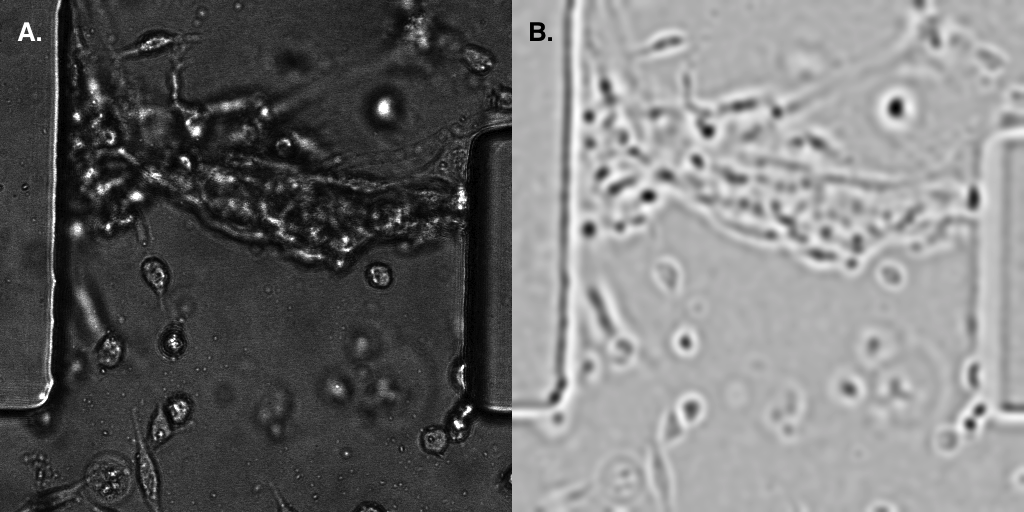
\includegraphics[width=0.9\textwidth]{303_sample_blobs}
 \caption[Sample of blob detection]{
 	Blobs, a technical term, are regions of contiguous (or interconnected) similar colours. Boundaries between these regions are edges and can be found using an appropriate filter as before. Blobs are found by convolving the image with a choice of filters. This image, A, was convolved with a simple Difference of Gaussians (DoG) curve. The size difference between the gaussians determines the scale of the blob that can be highlighted. Similarly sized blobs will give a similar ``response" and appear brighter in the final image, B.
 }
 \label{fig:blob}
\end{figure}

Once blobs and edges have been found, it is possible that in a given cellular environment, cells will be found packed closely in dense clusters. In order to be differentiated from each other, boundaries between the cells must be drawn based on the image properties surrounding them. Often, cells are separated by sharp discontinuities such as dark edges, but they may be so close that optically, their intensity curves appear to transition smoothly from one cell to another. In this case, a variant of the watershed method is useful for separating them [ref]. like many image processing techniques, the watershed method models the intensity map of the image as a terrain, where the contour height at a point is proportional to its intensity. If one imagines the terrain as being slowly filled with a certain amount of water, highly divergent regions such as cell representations will stand out like hills and the point where each ``hill" meets the water is the boundary of that cell. If the water is raised high enough, even smoothly transitioning boundaries between cells will appear to have a dividing line between them. This can be used to segment closely packed objects using their intensity peaks alone.

\begin{figure}[h!]
 \centering
 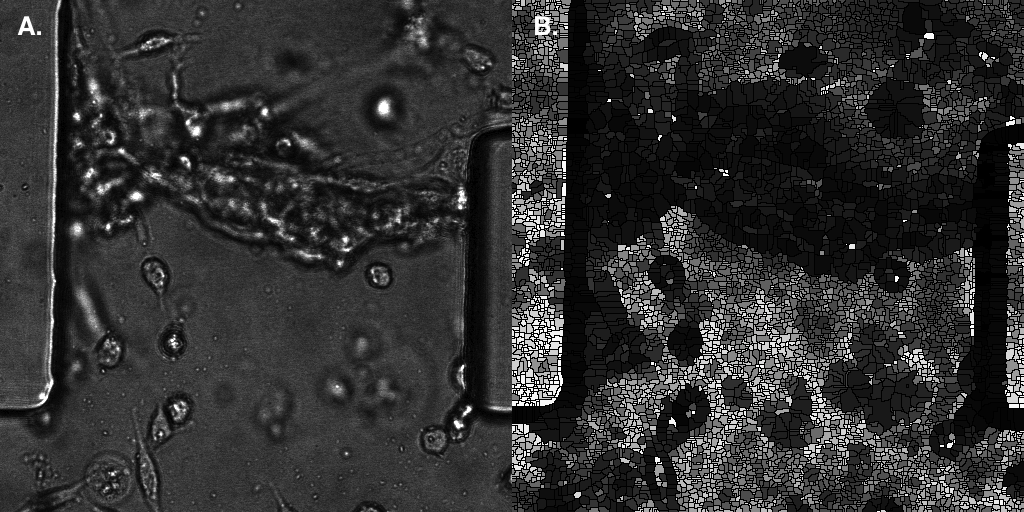
\includegraphics[width=0.9\textwidth]{304_sample_watershed}
 \caption[Watershed example]{
 	The watershed algorithm can be used to separate neighbouring objects by analysing the intensity curve joining their centres. If there is an inflection point in the intensity curve between them, it can be used to draw a line separating them. B shows an example of this type of algorithm applied to A, the original brightfield image. Parameters can be varied controlling the size of the objects separated to better estimate the types of curves that should be prioritised.
 }
 \label{fig:watershed}
\end{figure}

A watershed algorithm was proposed by F. Meyer in 1990. The steps for the watershed algorithm are as follows:
\begin{enumerate}
	\item Choosing starting points for the watershed. ``Water" will ``flow" from these points. These can be positioned at the maxima in an image, randomly, or in a grid. Each is given a different label (a simple integer value).
	\item Each iteration, the neighbours of the marked pixels are placed into a queue and ordered by a priority proportional to their grayscale values. There will be one queue per label.
	\item The neighbours of lowest priority pixel from each queue are checked. If they are all marked, the lowest priority pixel is marked with their label. Any un-queued neighbouring pixels are then queued.
	\item Repeat step 3 until all queues are empty.
\end{enumerate}

\section{CellProfiler and segmentation software}

The last section details some of the methods used by CellProfiler and other software packages, such as several ImageJ plugins, to segment cells. When CellProfiler is provided with an image, it will first look for blobs of colour in the image. Dependent on the background, it will look for bright or dark blobs as potential candidates for objects. The edges close to these blobs are kept as potential object edges. The blobs of colour are then separated using a watershed method. Their contours are matched with the edge image and the space is filled in to form an object ``mask". The mask is a binary representation the object of interest. Every point in the mask is considered part of the object, and all points outside are considered part of the background. The watershed method allows adjacent masks to be separated. Every task that CellProfiler performs on an image such as edge detection or blob detection is typically contained within a module that stores information about operations done to the image. These modules can be chained to compound effects and allow very specific workflows to suit all types of images. It can also combine images from several channels using basic mathematical operations.

\begin{figure}[h!]
 \centering
 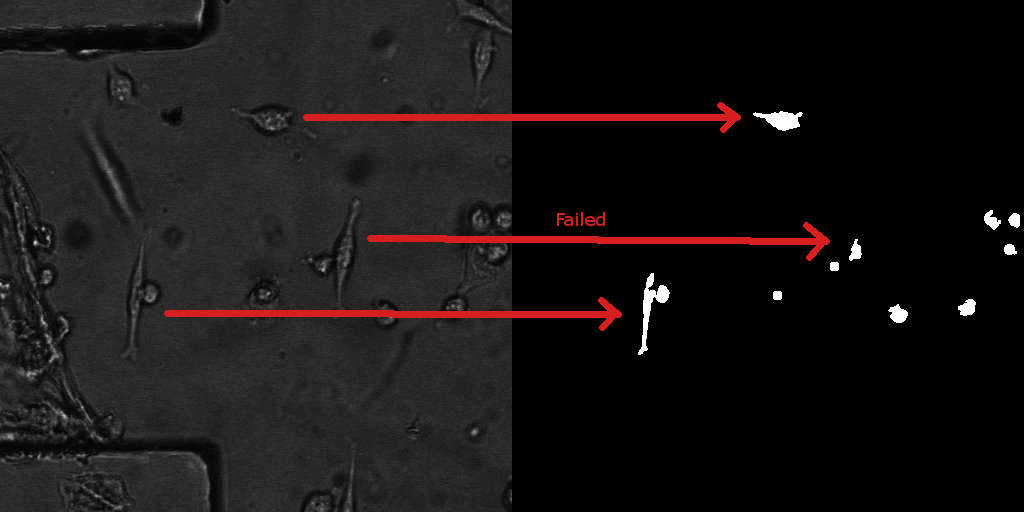
\includegraphics[width=0.9\textwidth]{305_masks}
 \caption[Object masks]{
 	A mask is the general term for a binary representation of an object. Pixels inside the mask, marked variously as white, true, 1, or 255, represent parts of the image that lie inside the object of interest. Pixels that are black, 0 or false, lie outside the object and are considered part of the background. If multiple objects are contained within the same mask image, they can be marked with a different integer such as 2, 23, 44, etc. to allow them to be differentiated. They may have previously been separated using a watershed algorithm or similar. By marking them with a unique grayscale id, they can be individually extracted from the image and observed. The examples given in B are typical outputs from cell recognisers such as CellProfiler.
 }
 \label{fig:masks}
\end{figure}

CellProfiler has a particularly useful module called ``Secondary Objects". Rather than searching the image for objects from scratch, it can use information about previously found objects to search in their vicinity. If object centres are represented as points, Secondary Objects can search around the points and use information about the vicinity of the point to match similar patches of colour or edge profiles. This operation is very adaptible, and does not have a size preference, filling whatever space is available. This is highly valued since one of the driving philosophies of this work is that recognition should not be biased towards a particular size or shape. A disadvantage of this approach is a recognition that expands without limit. If there is no discernible boundary, there is no reason for the recognition to stop expanding into the background if it is of similar intensity. To clarify, if the background of the image and the interior of the cell have similar colours, and the edges of the cell are incomplete or have an inconsistent profile, the recognition could add parts of the background to the final mask of the cell. This can affect the method used, but eventually adding 3D information to this 2D method can solve the problem.

\begin{figure}[h!]
 \centering
 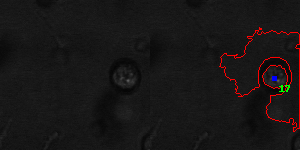
\includegraphics[width=0.9\textwidth]{308_secondary_objects_error}
 \caption[Secondary object error example]{
 	The Secondary Objects module in CellProfiler can caused errors in the recognition. In this case, the colour of the interior of the cell is very similar to that of the background. They are separated only by the dark colour of the edges. If there is a gap in the edge, or some interaction with exceptions at the edge of the image, the boundary separating the interior of the cell from the background can be poorly visible, allowing the segmentation to ``spill" from the previously marked interior into the background. This leads to results such as B. This causes the area or other numerical properties of the cell recognition to be overestimated and calls into question the utility of the recogniser.
 }
 \label{fig:secondaryobjecterror}
\end{figure}

Another tool for segmentation is the Blow/Lasso tool in ImageJ. This is based on the LASSO (or Least Absolute Shrinkage and Selection Operator) algorithm [ref]. LASSO is a least square regression algorithm that imposes a limit on...

NEED TO CORRECT THIS [???]

This treats the image as a ``terrain", where the ``height" of a pixel is proportional to its itensity. If an algorithm follows a path through the image, moving from one pixel to another can be assigned a cost based on the relationship between the intensities. An algorithm could be set up such that moving into dark edges could be very cheap, but moving out of them could be expensive, causing the path to follow a chain of edges closely. In a similar fashion, two points can be specified and the cost between them calculated [ref]. If one point is specified as the centre from which to search, the locus of points that share the same cost from the centre can yield a closed shape with dark edges such as a cell. While not reliable without tuning, the cost function can be made more specific to suit the application. Such a function can also be made to take account of multiple channels. Depending on how it is implemented, considering a central point can bias the shape towards a circular locus. Mathematically,

\begin{figure}[h!]
 \centering
 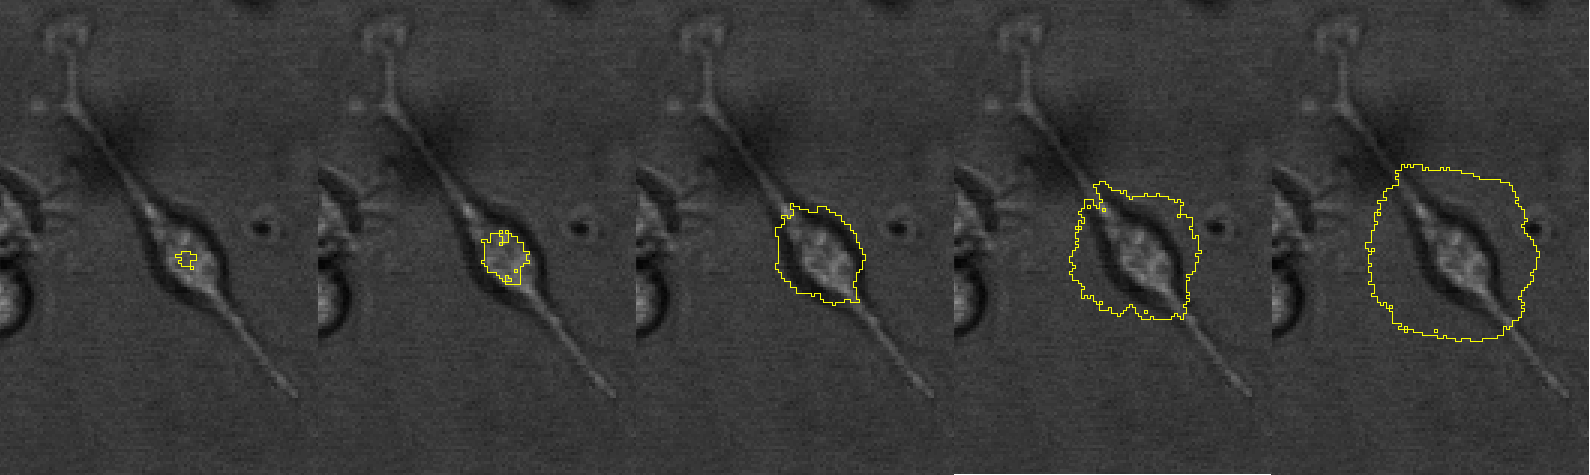
\includegraphics[width=0.9\textwidth]{309_blow_lasso}
 \caption[The LASSO tool]{
 	The LASSO algorithm, implemented in ImageJ as the Blow/Lasso tool, traverses the images from a centre to a test point and matches other points and paths in the image around that point that share the same ``energy". This can be used to closely fit the edges of an object, as the algorithm will avoid entering edges and other dark features. This can be used as a form of segmentation given a starting point.
 }
 \label{fig:blow}
\end{figure}

A notable disadvantage of CellProfiler is the lack of comprehensive support for 3D environments and sets of images with 3D relationships. Although it can be made to behave in this way, images must be processed on an individual basis or in basic groupings, limiting the complexity of 3D operations. This makes true 3D segmentation difficult or impossible. Nevertheless, CellProfiler has a wide array of very powerful 2D operations. Thus an ideal solution is a method that is able to cast a 3D dataset in a 2D context in order to take advantage of 2D methods while preserving 3D data.

The final data output from CellProfiler is a list of object masks along with some analysis [???] of their shape such as their eccentricity or orientation (from a bounding ellipse). CellProfiler does allow the segmentation of connected objects, such as protrusions, and can provide their measurements, but this can be unreliable since the properties of protrusions are hard to specify. A larger problem with CellProfiler is the inability to adapt to inconsistencies. For example, the edges of a cell protrusion can have a very different appearance to the main body of the cell as the cell walls grow thinner. A cell protrusion is defined as an extension or stretching of the cell wall used by the cell for movement. While the edge of a protrusion maybe remain visible towards its apex, the difference in edge properties might cause CellProfiler to conclude that they are unrelated edges, and lead to a protrusion being rejected and not represented in the final data. This unreliability with regards to ``tertiary object" like protrusions is insufficient for the accuracy required by this project. The method in Chapter [ref] will show how 3D information can enhance the recognition of tertiary objects.

\begin{figure}[h!]
 \centering
 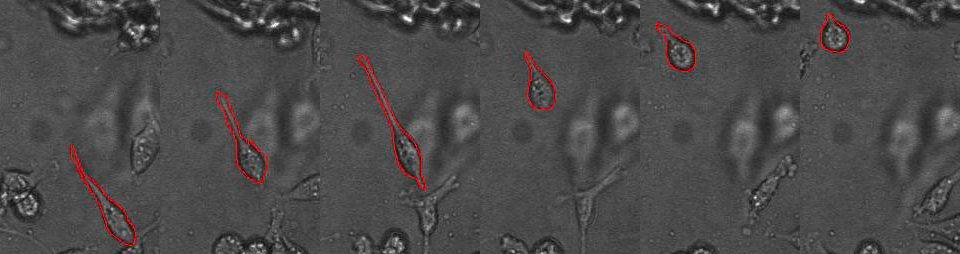
\includegraphics[width=0.9\textwidth]{310_protrusions}
 \caption[Cell protrusion example]{
 	The cell wall is a malleable series of interconnected proteins that can respond to a variety of chemical gradients. A typical response can take the form of a ``protrusion", which extends from the cell in a particular direction, usually in the direction of a stimulus. The cell depicted here is using the protrusion to move from the bottom of the image to the top. The protrusion first extends and then retreats as the movement is completed. Any useful cell recognition tool must allow such cell features to be tracked and measured. This is a key goal of this study.
 }
 \label{fig:cellprotrusions}
\end{figure}

\section{Cell tracking}

Cell tracking is any method of associating recognised objects in different images gathered at different times and assigning them same identity. This can allow properties of the cells such as area and position to be plotted over time and for trends to be observed. In a low density packing of cells, this can be as simple as finding the distance between objects in different frames and assigning the next iteration to be the object with the smallest distance from the starting point. In this study, connected iterations of a single physical object are referred to as ``instances" as in ``cell instance". This is an important distinction, since a cell objects cannot be said to have an area or velocity since these properties change with time. Velocity also requires multiple frames to determine, so intermediate velocities can be assigned to the cell instance rather than the cell. Assigning an area to a particular cell at a point in time is equivalent to assigning the area to the cell instance. Thus a single cell can have many cell instances.

A popular tracking method is the LAP, or ``Linear Assignment Problem", framework tracking algorithm. Once two lists of objects and their positions in subsequent images are found, they can be connected and ranked by a likelihood of correspondence. This is done by first constructing and solving a NxN [maths] matrix of correspondence parameters where N is the number of objects considered. A similar matrix is constructed to represent the probabilities of cells merging or splitting. The final step reconciles the two images into a list of corresponding cell instances. This process can then be repeated for subsequent frames. This algorithm is employed by CellProfiler as a module, so it can be applied to objects found through recognition. Other properties of the cells such as changing shape and size can contribute to the likelihood of correspondence. LAP also helps to associate cells that disappear and reappear, as well as cells that merge or split.

The method yields four important numbers, namely ``LostObjectCount", ``NewObjectCount", ``SplitObjectCount", and ``MergedObjectCount". A measure of the reliability of the tracking is given by the consistency of these numbers. For example, if NewObjectCount continues to increase throughout the time series, it is likely that objects that should be connected are being rejected and treated as new objects. This can happen if objects move a long distance, such as many multiples of their length, between frames. If the ratio of distance moved to time between frames is too high, the tracking algorithm may be too unreliable for use. Due to this unreliability, manual tracking is necessary to provide accurate information about cells. Manual tracking is used throughout this study, but further possiblities for automatic tracking can be derived from the current research.

\section{The Selinummi brightfield profile method}

In their 2009 paper, Bright Field Microscopy as an Alternative to Whole Cell Fluorescence in Automated Analysis of Macrophage Images [italic], Selinummi et al. describe a method of using 3D brightfield information to aid segmentation instead of relying on GFP imaging of cells. The images for their study were gathered in a similar way to this study. A confocal microscope was used to scan a 3D environment gathering images in brightfield and GFP channels. Gathering data with a confocal microscope is slow and expensive, so if adequate cell data can be produced using a single channel, this can save time. They proposed using the amplitude of the variation of the brightfield intensity in the Z dimension as an indicator of the presence of an object at a particular XY location. This exploits the behaviour of the brightfield representations of objects as they move in and out of focus. As outlined in Chapter [ref], the brightfield does not store 3D information, but changes with the focal plane of the environment. An area of background will not vary across focal planes, but a location or single pixel containing an object will vary with focal plane.

The basis of the method is an inspiration for the current project. The vertical distribution of the brightfield intensities at a particular XY location, known as a ``profile" in this study, shows how the features vary in intensity across Z.

\begin{figure}[h!]
 \centering
 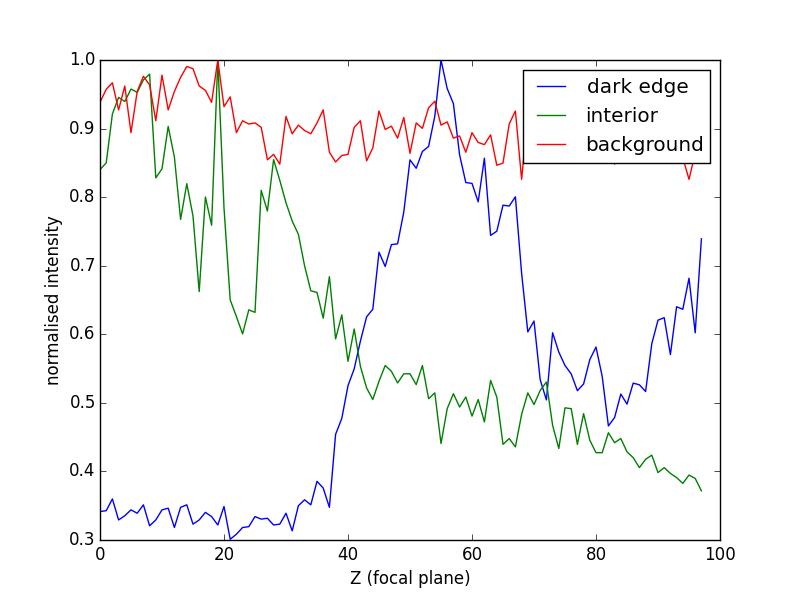
\includegraphics[width=0.9\textwidth]{311_bf_profiles}
 \caption[Selinummi brightfield profile]{
 	The brightfield profile was shown by Selinummi et al. to be a powerful indicator of the presence of an object in an image. The profile for each pixel in XY is the intensity distrbution of the column of pixels in Z. For three typical points in an image of a cell, A, the background, the edge of a cell, and the interior of a cell have very different profiles, seen in B. These differences can be used to separate parts of the image that can contain cells from those that contain only background.
 }
 \label{fig:brightfieldprofile}
\end{figure}

Their results were promising for the data they gathered, but suffered when applied to the data from the current experiment. To test the method, they compared cell segmentation of the modified brightfield images to the GFP images of the same cells. They used the GFP segmentation as the ``ground truth" of their testing. Ground truth is assumed to be the best representation of the object. This is a failing of the study since there are many details omitted by the GFP, especially considering the variety of configurations cellular GFP can take. Segmentation was compared pixel by pixel using the ``FScore", or a compound ratio of the true and false positive scores, given by:
$$ Precision = \frac{tp}{tp + fp} $$
$$ Recall = \frac{tp}{tp + fn} $$
$$ FScore = \frac{2 (Precision \times Recall) }{Precision + Recall} $$
where:
\begin{enumerate}
	\item $tp$ is the number of True Positive, or correctly recognised pixels in a mask, according to the ground truth, or accepted best measurement of the cell.
	\item $fp$ is False Positive, or falsly accepted pixels.
	\item $fn$ is False Negative, or pixels falsly rejected from the mask.
\end{enumerate}
FScore serves as a means of judging the accuracy of a mask from a certain algorithm in one single value.

There are several disadvantages of the Selinummi method, especially when applied to the current data. Firstly, the method was originally applied to a single cell environment with no visible materials other than cells. In contrast, the current environment is primarily composed of PDMS plastic. It is also a multicellular environment. The images thus contain many other objects in the brightfield that are not desired as part of the dataset, but they still have similar edges and strong variations in their intensity profiles. Regions of the image where any kind of object is found will appear bright. This can hinder accurate segmentation since unwanted objects are highlighted. Secondly, due to the brightfield variation in the images, strongly varying pixels can occur outside the true edge of the cell, causing these regions to be highlighted, and giving the cell a bright halo. This halo is picked up in the recognition and contributes to the measured area of the cell. This can cause an over-estimation of the cell area and a false representation of the cell's shape. These problems must be addressed for a variant of this method to be useful.
